\chapter{直线、平面坐标化}
\section{直线坐标化}

\subsection{直线的有向化}
在日常生活或科学研究中,往往需要考虑直线的方向。
凡具有方向的直线称为有向直线,给直线以一定的方向就是
将直线有向化,一条直线含有两个相反的方向,所以一条直
线有两种相反的有向化。

例如,北京市的长安街有西、东之分;在街上奔驰的车
辆有往、返之别。

在任一条直线上,可以规定它的某一方向作为正向,它
的另一方向则作为负向。在数学里,一般是规定直线的向上
方向或向右方向为正向,向下方向或向左方向为负向,如图
2.1。
\begin{figure}[htp]
    \centering
\begin{tikzpicture}[>=latex]
\draw[<->] (0,0)node [right]{负向} --(0,3)node [right]{正向};
\draw[<->] (2.5,1.5)node [below]{负向} --(5,1.5)node [below]{正向};
\end{tikzpicture}
    \caption{}
\end{figure}

每条线段都有两个端点,如果把一个端点取做始点,另
一个端点取做终点,由始点到终点的方向叫做该“有向线段”
的方向。如果它的方向和它所位于的有向直线的方向一致,
则它是一个正向线段;如果它们的方向相反则它是一个负向
线段。因此,可以说一条线段有两个相反的方向。凡是考虑
方向的线段,称为有向线段。例如,在有向直线$\ell$上取$A,B$
两点(图2.2),则有向线段$AB$是正向线段,有向线段$BA$是
负向线段。
\begin{figure}[htp]
    \centering
\begin{tikzpicture}[>=latex]
\draw[->] (0,0) --(5,0)node[right]{$\ell$};
\draw (1.5,0)[fill=black] circle (1.5pt)node[below]{$A$};
\draw (3.5,0)[fill=black] circle (1.5pt)node[below]{$B$};
\end{tikzpicture}
    \caption{}
\end{figure}

表示有向线段,一般是将始点写在终点的左边,并在两
个字母上面加一个箭头。如以$A$为始点,$B$为终点的有向线
段记作$\Vec{AB}$, 以$B$为始点。$A$为终点的有向线段记为$\Vec{BA}$。

我们可以用一个有正负号的实数来同时表达在有向直线
上的有向线段的长度和它的正、负方向。这个实数称为该有
向线段的数量。

如图2.2. 设有向线段$\Vec{AB}$的数量是$\alpha\; (\alpha>0)$, 则有向线
段$\Vec{BA}$的数量是$-\alpha$。有时也用$AB$表示有向线段$\Vec{AB}$的数量,用
${BA}$表示有向线段$\Vec{BA}$的数量。显然有向线段$\Vec{AB}$与$\Vec{BA}$的数量
有下列关系:
\[AB=-BA\]
或\[AB+BA=0\]

符号
$|\Vec{AB}|$表示只考虑有向线段$\Vec{AB}$的长度而不考虑方
向。符号$|\Vec{AB}|$也称有向线段$\Vec{AB}$的数量的绝对值。

\subsection{直线的坐标化}
规定了方向,规定了基准点或原点,并规定了长度单位
的直线,称为\textbf{数轴}。这就是直线的坐标化,如图2.3,在日常
生活中,用直尺上的刻度表示长度的大小,用温度计上的刻
度表示温度的高低,这实际上就是把实数$\pm a$对应于数轴上一
点,这点和原点距离等于$a\; (a\ge 0)$, 由于数轴是连续不间断
的,所有的实数,都能用数轴上的点表示出来。在数轴上,
数0用原点表示,正数对应着原点右方的点,负数对应着
原点左方的点。

\begin{figure}[htp]
    \centering
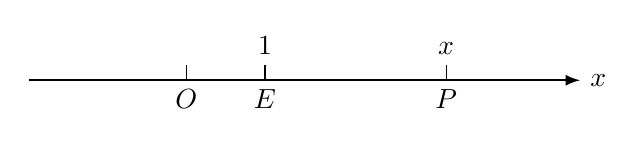
\begin{tikzpicture}[>=latex]
\draw[thick, ->] (-2,0)--(5,0)node[right]{$x$};
\foreach \x in {0,1,3.3}
{
    \draw(\x,0)--(\x,0.2);
}
\node at (0,0) [below]{$O$};
\node at (1,0) [below]{$E$};
\node at (3.3,0) [below]{$P$};
\node at (1,0.2) [above]{$1$};
\node at (3.3,0.2) [above]{$x$};

\end{tikzpicture}
    \caption{}
\end{figure}

\begin{example}
    把下列各数用数轴上的点表示出来:
\[2,\quad -2,\quad -3.5,\quad 3.5,\quad \sqrt{2},\quad \sqrt{3}\]
\end{example}

\begin{solution}
    先画数轴,然后在数轴上找出相应的点。
图2.4中的$A,B,C,D,E,F$分别表示$2,\; -2,\; -3.5,\; 
3.5,\; \sqrt{2},\; \sqrt{3}$。

\begin{figure}[htp]
    \centering
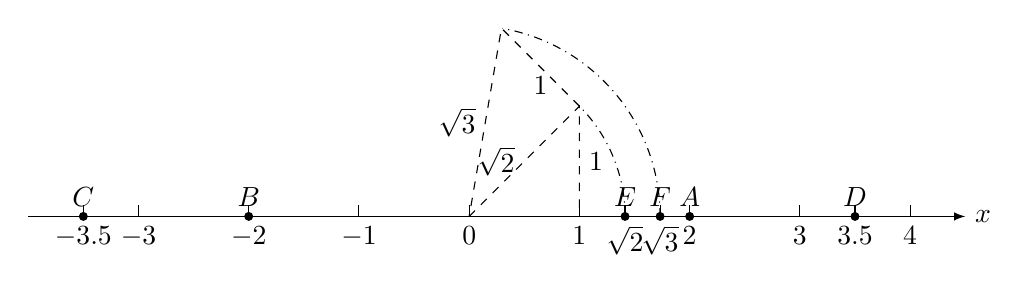
\begin{tikzpicture}[>=latex, scale=1.4]
\draw[->] (-4,0)--(4.5,0) node[right]{$x$};
\foreach \x/\xtext in {2/A,-2/B,-3.5/C,3.5/D,1.414/E,1.732/F}
{
    \draw (\x,0)--(\x,.1);
    \draw (\x,0)[fill=black] circle (1pt);
    \node at (\x,0) [above]{$\xtext$};
}

\foreach \x in {2,-2,-3.5,3.5}
{
    \node at (\x,0) [below]{$\x$};
}

\foreach \x in {-3,-1,0,1,3,4}
{
    \draw (\x,0)--(\x,.1);
    \node at (\x,0) [below]{$\x$};
}
\node at (1.414,0)[below]{$\sqrt{2}$};
\node at (1.732,0)[below]{$\sqrt{3}$};

\draw[dashed] (0,0)--node[left]{$\sqrt{2}$}(1,1)--node[right]{1}(1,0);
\draw[dashdotted] (1.414,0) arc (0:45:1.414);

\draw[dashed]  (1,1)--node[below]{1}(1-1/1.414, 1+1/1.414)--node[left]{$\sqrt{3}$}(0,0);
\draw[dashdotted] (1.732,0) arc (0:80:1.732);
\end{tikzpicture}
    \caption{}
\end{figure}
\end{solution}


反过来,在数轴上每取一点$P$(图2.3), 有向线段$\Vec{OP}$总是
单位有向线段$\Vec{OE}$的实数倍;即存在一个实数$x$, 使得
\[\Vec{OP}=x\Vec{OE} \]
如果$P$点和$E$点在原点同侧,则$x>0$; 如果$P$点和$E$点在原点
异侧,则$x<0$. 从上述两方面看,数轴上的点与实数之间可以
建立一一对应。因此,在直线上建立数轴后,就形成直线的一
个坐标系,实数$x$叫做$P$点的坐标。换言之,数轴上一个点$P$
的坐标就是以原点为始点,以该点为终点的有向线段$\Vec{OP}$的数
量。

如图2.4, $F$点的坐标是$\sqrt{3}$, 而有向线段$\Vec{OF}$的数量是
$\sqrt{3}$; $C$点的坐标是$-3.5$, 而有向线段$\Vec{OC}$的数量是$-3.5$. 即$OF=\sqrt{3}$; $OC=-3.5$.

从图2.4中可以看出,和原点距离相等的两个点,如点$A$
和点$B$, 点$C$和点$D$, 它们所表示的数分别是2和$-2$; $-3.5$
和3.5。这样的数称为相反数。

根据相反数的概念,一个实数的绝对值曾规定如下:
\begin{blk}{}
    正数或零的绝对值是它们自己;
负数的绝对值是它的相反数。
\end{blk}

用符号表示如下:
\[|x|=\begin{cases}
    x, & x\ge 0\\
    -x, & x<0
\end{cases}\]

借助于数轴,我们可以对一个数的绝对值作出几何解
释:把这个数用数轴上的点表示出来,那么这个数的绝对值
就是原点到表示这个数的点的距离。从这里看出,除零以外,
正数和负数的绝对值都是正数,而且两个相反数的绝对值相
等。

前面已说明在数轴上的一点$P$的坐标$x$就是以原点$O$为始
点,以$P$点为终点的有向线段$\Vec{OP}$的数量$OP=x$。

现在进一步研究在数轴上任意一条有向线段的数量表示
法;在数轴上任取不同的两点$A,B$, 设$A$点的坐标为$x_1$, $B$
点的坐标为$x_2$. 如图2.5(1), 现在要求$AB=?$

由图看出:$|\Vec{OB}|=|\Vec{OA}|+|\Vec{AB}|$
故得
\[|\Vec{AB}|=|\Vec{OB}|-|\Vec{OA}|\]
$\because\quad \Vec{AB}, \Vec{OB}, \Vec{OA}$都是正有向线段,

$\therefore\quad AB=OB-OA=x_2-x_1$

当然,$A,B$两点在数轴上的位置不只如图2.5(1)的那
样一种,还有图2.5(2)--(6)几种情况。

\begin{figure}[htp]
    \centering
    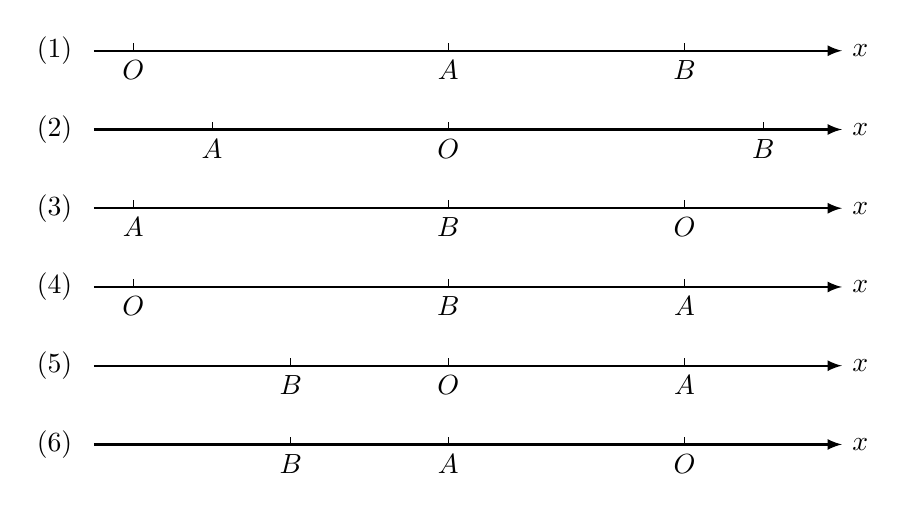
\begin{tikzpicture}[>=latex]
\foreach \y in {-1,-2,...,-6}
{
    \draw[->, thick](-4.5,\y)--(5,\y)node[right]{$x$};
}
\foreach \x/\xtext in {-4/O,0/A,3/B}
{
    \draw (\x,-1)--(\x,-1+.1);
    \node at (\x,-1)[below] {$\xtext$};
}
\foreach \x/\xtext in {-3/A,0/O,4/B}
{
    \draw (\x,-2)--(\x,-2+.1);
    \node at (\x,-2)[below] {$\xtext$};
}
\foreach \x/\xtext in {-4/A,0/B,3/O}
{
    \draw (\x,-3)--(\x,-3+.1);
    \node at (\x,-3)[below] {$\xtext$};
}
\foreach \x/\xtext in {-4/O,0/B,3/A}
{
    \draw (\x,-4)--(\x,-4+.1);
    \node at (\x,-4)[below] {$\xtext$};
}
\foreach \x/\xtext in {-2/B,0/O,3/A}
{
    \draw (\x,-5)--(\x,-5+.1);
    \node at (\x,-5)[below] {$\xtext$};
}
\foreach \x/\xtext in {-2/B,0/A,3/O}
{
    \draw (\x,-6)--(\x,-6+.1);
    \node at (\x,-6)[below] {$\xtext$};
}
\node at (-5,-1){(1)};\node at (-5,-2){(2)};
\node at (-5,-3){(3)};\node at (-5,-4){(4)};
\node at (-5,-5){(5)};\node at (-5,-6){(6)};
    \end{tikzpicture}
    \caption{}
\end{figure}



但不管哪一种情况,都可证得$AB=x_2-x_1$。譬如在图2.5
的(2)中,$AB=|\Vec{AB}|$, $OA=-|\Vec{OA}|$, $OB=|\Vec{OB}|$, 而
\[|\Vec{AB}|=|\Vec{OA}|+|\Vec{OB}|\]
$\therefore\quad AB=-OA+OB$,就是
\[AB=OB-OA=x_2-x_1\]

其它情形,同样地可以证明,这就是说,\textbf{在数轴上任意一
条有向线段的数量等于其终点坐标与始点坐标的差}。

\section*{习题2.1}
\addcontentsline{toc}{subsection}{习题2.1}
\begin{enumerate}
    \item 在数轴上$A,B$两点的坐标分别是$x_1,x_2$, 设:
\begin{multicols}{2}
\begin{enumerate}
    \item $x_1=-2,\quad x_2=2$
    \item $x_1=-9,\quad x_2=-11$
    \item $x_1=-3,\quad x_2=5$
    \item $x_1=0,\quad x_2=-8$
\end{enumerate}
\end{multicols}
试求有向线段$AB$与$BA$的数量以及$|AB|,\; |BA|$

\item 若$A,B,C$是数轴上任意三个点,它们的坐标分别是$a,
b,c$, 求证:$AB+BC+CA=0$
\item 若$A,B$两点坐标各为$a,b$, 求:
\begin{enumerate}
    \item 中点$C$的坐标,
    \item 二个三等分点的坐标。
\end{enumerate}

\item 
在数轴上确定坐标是$2+\sqrt{2}$, $3-\sqrt{3}$, $\sqrt{5}$, $\sqrt{6}$的点。
\item 
设数轴上的$P$点的坐标$x$满足条件:
\begin{enumerate}
    \item $|x|=2$
    \item $|x-1|=5$
    \item $|2x+1|=5$
\end{enumerate}
求$P$点的坐标。
\item 如果在一个杆子上的两点$A,B$分别挂上重量等于$p$, $q$公
斤的物品,假设$A,B$的坐标分别是$a,b$, 试问支点(也就
是重心)的坐标应该是多少才能平衡(假定杆子的重量可
以忽略不计)。


\end{enumerate}

\section{平面的坐标化}

\subsection{平面的直角坐标化}
在平面上取一定点$O$作为基准点,或称为原点,过原点引
两条互相垂直的数轴。图2.6是常用的取法,把一条数轴取
为水平方向,称为横轴,或叫做$x$轴,以向右为正向;另一
条数轴取为铅垂方向,称为纵轴,或叫$y$轴,以向上为正向。
上述的取法称为在平面内建立直角坐标系,利用直角坐标
系,我们可以用一对有序的实数来表示平面内一个点的位
置。

\begin{figure}[htp]
\centering
\begin{minipage}[t]{0.48\textwidth}
\centering
\begin{tikzpicture}[>=latex, scale=.7]
    \draw[->,thick] (-3,0)--(3,0) node[right]{$x$};
    \draw[->,thick]  (0,-3)--(0,3)node[right]{$y$};
\node at (-.3,-.3){$O$};
\node at (1.5,1.5){一};\node at (-1.5,1.5){二};
\node at (-1.5,-1.5){三};\node at (1.5,-1.5){四};
\node at (1.5,1){$(+,+)$};\node at (-1.5,1){$(-,+)$};
\node at (-1.5,-2){$(-,-)$};\node at (1.5,-2){$(+,-)$};
\end{tikzpicture}
\caption{}
\end{minipage}
\begin{minipage}[t]{0.48\textwidth}
\centering
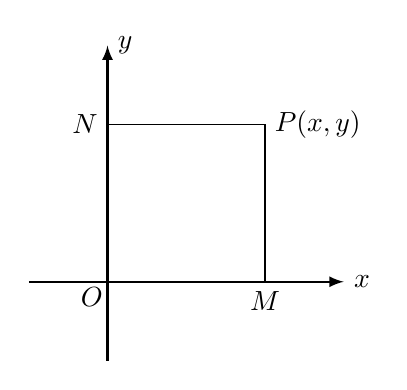
\begin{tikzpicture}[>=latex]
    \draw[->,thick] (-1,0)--(3,0)node[right]{$x$};
    \draw [->,thick] (0,-1)--(0,3)node[right]{$y$};
    \node at (-.2,-.2){$O$};
\draw (2,0)node[below]{$M$}--(2,2)node[right]{$P(x,y)$}--(0,2)node[left]{$N$};

\end{tikzpicture}
\caption{}
\end{minipage}
\end{figure}



在平面上任取一点$P$(图2.7), 过点$P$分别作$y$轴,$x$轴的平
行线$PM$, $PN$, 于是得到有向线段$\Vec{OM}$, $\Vec{ON}$, 而有向线段$\Vec{OM}$, $\Vec{ON}$分别在$x$轴,$y$轴上的数量是$x,y$, 也就是说,在平面上
任取一点$P$, 可以找到与之对应的一对实数$x,y$。反过来说,
任取一对实数$x,y$, 在$x$轴,$y$轴上可以分别找到与之对应
的以原点$O$为始点,以$M,N$为终点的有向线段$\Vec{OM}$, $\Vec{ON}$,
过$M,N$各作$y$轴、$x$轴的平行线,这两条平行线必交于与之
对应的一点$P$. 这样,平面内的点和所有的有序实数对$(x,y)$之间就建立了一一对应的关系。我们就用这样一对有序实
数$x,y$作为点$P$在平面内位置的标记,称为点$P$的坐标。

有向线段$\Vec{OM}$的数量$x$称为点$P$的横坐标或横标,有向线
段$\Vec{ON}$的数量$y$称为点$P$的纵坐标或纵标,点$P$的坐标记为$(x,
y)$。

横、纵两轴把平面分为四部分,按逆时针次序分别叫做
第一象限、第二象限、第三象限和第四象限。显然,在第一
象限点的横标、纵标都是正数;在第二象限点的横标为负,纵
标为正;在第三象限点的横标、纵标都是负数;在第四象限
点的横标为正、纵标为负。反过来也对(图2.6)。

通过坐标系的建立,可以把平面内的点和有序实数对
$(x,y)$一一对应起来,这就有可能把平面内关于点的几何问
题,化成关于这些点的坐标的代数的问题来进行研究。这也
就是用代数方法即解析方法来解决几何问题。

\begin{example}
    菱形的每边长为5, 一条长对角线为8, 如果以
    菱形的对角线作为坐标轴,试求此菱形各顶点的坐标,并描
    绘出菱形的图形。
\end{example}

\begin{solution}
    因为菱形的对角线互相垂直平分。设菱形顶点分别
为$A,B,C,D$. 根据已知条件,设长对角线在$x$轴上,则知
$A,C$坐标各为$(4,0)$, $(-4,0)$. 设$B,D$坐标各为$(0,b)$,
$(0,-b)$。

$\therefore\quad |AB|=BC|=|CD|=|DA|=5$

由勾股定理可求得$B,D$的坐标各为$(0,3)$, $(0,-3)$.

同理可得另一种情形:(图2.8)
\[A(3,0),\quad B(0,4),\quad C(-3,0),\quad D(0,-4)\]
\begin{figure}[htp]
    \centering
    \begin{tikzpicture}[>=latex, scale=.5]
\begin{scope}
    \draw[->](-5,0)--(5,0)node[right]{$x$};
    \draw[->](0,-4)--(0,4)node[right]{$y$};
    \node at (-.4,-.4){$O$};
\draw (-4,0)node[above]{$C$}--(0,3)node[right]{$B$}--(4,0)node[above]{$A$}--(0,-3)node[right]{$D$}--(-4,0);
\end{scope}

\begin{scope}[xshift=12cm]
    \draw[->](-4,0)--(4,0)node[right]{$x$};
    \draw[->](0,-5)--(0,5)node[right]{$y$};  
    \node at (-.4,-.4){$O$};
    \draw (-3,0)node[above]{$C$}--(0,4)node[right]{$B$}--(3,0)node[above]{$A$}--(0,-4)node[right]{$D$}--(-3,0);
\end{scope}
    \end{tikzpicture}
    \caption{}
\end{figure}

\end{solution}

\begin{example}
  一船向北偏东$60^{\circ}$航行40公里,再向北偏东$45^{\circ}$航
行24公里,这时船在起点东面多少公里?北面多少公里(精确
到1公里)?  
\end{example}

\begin{figure}[htp]
    \centering
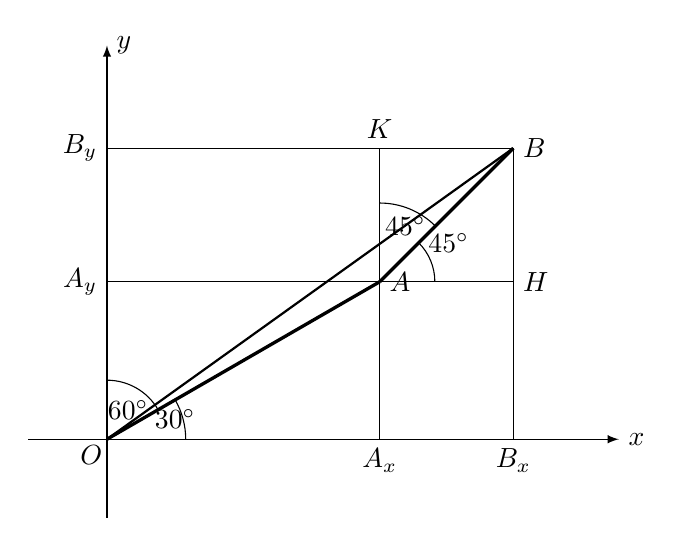
\begin{tikzpicture}[>=latex]
\draw[->](-1,0)--(6.5,0)node[right]{$x$};
\draw[->] (0,-1)--(0,5)node[right]{$y$};
\draw (2*1.732,0)node[below]{$A_x$}--(2*1.732, 2)node[right]{$A$}--(0,2)node[left]{$A_y$};
\draw (2*1.732+1.2*1.414,0)node[below]{$B_x$}--(2*1.732+1.2*1.414, 2)node[right]{$H$}--(2*1.732+1.2*1.414, 2+1.2*1.414)node[right]{$B$}--(2*1.732,2+1.2*1.414)node[above]{$K$}--(0,2+1.2*1.414)node[left]{$B_y$};
\node at (-.2,-.2){$O$};
\draw (2*1.732+1.2*1.414, 2) rectangle(2*1.732,2+1.2*1.414);

\draw[very thick] (0,0) -- (2*1.732, 2);
\draw[ thick] (0,0) -- (2*1.732+1.2*1.414, 2+1.2*1.414);
\draw[very thick] (2*1.732, 2) -- (2*1.732+1.2*1.414, 2+1.2*1.414);

\draw(1,0)  arc (0:30:1) node[below]{$30^{\circ}$};
\draw(0,.75) arc (90:30:.75)node[left]{$60^{\circ}$};
\draw (2*1.732+.7, 2) arc (0:45:.7) node[right]{$45^{\circ}$};
\draw (2*1.732, 3) arc (90:45:1) node[left]{$45^{\circ}$};


\end{tikzpicture}
    \caption{}
\end{figure}


\begin{solution}
    建立直角坐标系$x-O-y$, 如图2.9。设起点在原点
$O$,$y$轴代表正北方向,$x$轴代表正东方向,船向北偏东$60^{\circ}$航行40公里的位移用有向线段$\Vec{OA}$代表,再向北偏东$45^{\circ}$航行24公
里的位移用有向线段$\Vec{AB}$代表,这时船在$B$点的坐标是$(x,y)$.

因为$A$点的横坐标$x_A$是有向线段$\Vec{OA}$在$x$轴上的射影$\Vec{OA}_x$的数量,即
\begin{equation}
\begin{split}
      x_A=OA&=|OA|\cos(90^{\circ}-60^{\circ})\\
    &=  40\cos 30^{\circ}\\
    &=20\sqrt{3}
\end{split}
\end{equation}
$A$点的纵坐标$y$是有向线段$\Vec{OA}$在$y$轴上的射影$\Vec{OA}_y$的数量,即
\begin{equation}
    \begin{split}
y_A=OA&=|OA|\cos60^{\circ}\\
&=40\cos60^{\circ}\\
&=40\x\frac{1}{2}=20        
    \end{split}
\end{equation}

又有向线段$\Vec{AB}$在$x$轴上的射影$\Vec{A_xB_x}$的数量是
\begin{equation}
A_xB_x=AH=|AB|\cos45^{\circ}=24\x\frac{\sqrt{2}}{2}=12\sqrt{2}        
\end{equation}
有向线段$\Vec{AB}$在$y$轴上射影的数量是
\begin{equation}
    A_yB_y=AK=|AB|\cos45^{\circ}=24\x\frac{\sqrt{2}}{2}=12\sqrt{2}        
    \end{equation}

另一方面,
\[\begin{split}
    A_xB_x&=OB_x-OA_x=x-x_A=x-20\sqrt{3}\\
    A_yB_y&=OB_y-OA_y=y-y_A=y-20 
\end{split}\]
将(2.3), (2.4)分别代入上面两个等式的左端,得
\[\begin{cases}
    12\sqrt{2}=x-20\sqrt{3}\\
    12\sqrt{2}=y-20
\end{cases}\]
因此:
\[\begin{split}
    x&=20\sqrt{3}+12\sqrt{2}\approx 20\x 1.73+12\x 1.41 \approx 51.55\approx 52\\
    y&=20+12\sqrt{2}\approx 20+12\x 1.41\approx 36.9\approx 37
\end{split}\]
答:船在起点东面约52公里,在北面约37公里的地方。
\end{solution}

\begin{ex}
\begin{enumerate}
    \item 正方形的边长为$b$, 对角线在坐标轴上,试求各顶点的
    坐标。
    \item 已知矩形相邻两边的长分别为$a,b$, 各在$x$轴及$y$轴上,
    试求其各顶点坐标。
    \item 已知正方形的边长为$2a$, 一顶点为原点$O\;(0,0)$, 一对角线
    在$x$轴的正方向上,试求其它顶点的坐标。
    \item 正三角形的边长为$b$, 一顶点为原点$O\;(0,0)$, 其高在$y$
    轴上,试求其余两顶点的坐标。
    \item 有一边长是$a$的正三角形$ABC$, $AB$边在$x$轴上,$AB$边的
    中点是原点,试求$\triangle AEC$各顶点的坐标。
    \item 在平行四边形$ABCD$中,$|AB|=8$, $|AD|=5$, $\angle A=
    60^{\circ}$, 如果以点$A$为原点,$AB$所在直线为$x$轴,$C$点所在
    象限为第一象限,试求各顶点的坐标。
\end{enumerate}
\end{ex}

\subsection{两点间的距离}
若两点为$P_1\;(x_1,y_1)$, $P_2\;(x_2,y_2)$, 则这两点间的距离为;
$$|\Vec{P_1P_2}|=\sqrt{(x_2-x_1)^2+(y_2-y_1)^2}$$

\begin{figure}[htp]
    \centering
\begin{tikzpicture}[>=latex,scale=.6]
    \draw[->](-5,0)--(5,0)node[right]{$x$};
    \draw[->] (0,-4)--(0,5)node[right]{$y$};
\draw[dashed](-4,0)node[above]{$M_1$}--(-4,-3)--(0,-3)node[right]{$N_1$}--(3,-3)node[right]{$S$}--(3,0)node[above]{$M_2$}--(3,4)--(0,4)node[left]{$N_2$};
\draw[very thick](-4,-3)node[left]{$P_1$}--(3,4)node[right]{$P_2$};
\node at (-.3,-.3){$O$};
\end{tikzpicture}
    \caption{}
\end{figure}



事实上,由$P_1$, $P_2$引$y$轴、$x$轴的平行线$P_1M_1$, $P_2M_2$,
$P_1N_1$, $P_2N_2$, 延长$P_1N_1$与$P_2M_2$相交于$S$(图2.10), 在直角三角形$P_1SP_2$中,由勾股定理得:
\[|\Vec{P_1P_2}|^2=|\Vec{P_1S}|^2+|\Vec{SP_2}|^2 \]
其中,$|\Vec{P_1S}|=|\Vec{M_1M_2}|=|x_2-x_1|$,$|\Vec{SP_2}|=|\Vec{N_1N_2}|=|y_2-y_1|$。

于是$$|\Vec{P_1P_2}|^2=|x_2-x_1|^2+|y_2-y_1|^2$$
开平方得:
$$|\Vec{P_1P_2}|=\sqrt{(x_2-x_1)^2+(y_2-y_1)^2}$$
这就是平面上任意两点间的距离公式。

有了两点间距离公式,我们还可以把实数的绝对值和算
术平方根的概念联系起来,把两点间距离公式应用到点
$P\; (x,0)$和原点$(0,0)$上,得
\[d=\sqrt{(x-0)^2+(0-0)^2}=\sqrt{x^2}\]
但另一方面,在$x$轴上表示数$x$的$P$点到原点的距离就是$|x|$, 
因此
\[|x|=\sqrt{x^2}\]
这表示一个数的绝对值就等于这个数的平方的算术平方根。

\begin{example}
    试求两点$A(e,a)$, $B(e,b)$间的距离。
\end{example}

\begin{solution}
    设$x_1=e$, $y_1=a$, $x_2=e$, $y_2=b$, 由距离公式可得:
\[|\Vec{AB}|=\sqrt{(e-e)^2+(b-a)^2}=|b-a|\]
\end{solution}

\begin{example}
    试求$P(c,f)$, $Q(d,f)$两点间的距离。
\end{example}


\begin{solution}
    设$x_1=c$, $y_1=f$, $x_2=d$, $y_2=f$, 由两点间的距离
公式可得
\[|\Vec{PQ}|=\sqrt{(d-c)^2+(f-f)^2}=\sqrt{(d-c)^2}=|d-c|\]
\end{solution}

由以上两例可以看出,如果两点间的线段平行于$x$轴或
$y$轴,则其距离分别等于这两点横标、纵标的差的绝对值。


\begin{example}
    已知$\triangle ABC$各顶点为$A(-\sqrt{3},\sqrt{2})$,
$B(-\sqrt{2},\sqrt{3})$, $C(\sqrt{3},\sqrt{2})$, 试求此三角形三边的长。
\end{example}

\begin{solution}
$\because\quad A(-\sqrt{3},\sqrt{2}),\qquad B(-\sqrt{2},\sqrt{3})$

$\therefore\quad |\Vec{AB}|=\sqrt{\left(-\sqrt{2}+\sqrt{3}\right)^2+\left(\sqrt{3}-\sqrt{2}\right)^2}=\sqrt{10-4\sqrt{6}}$

$\because\quad B(-\sqrt{2},\sqrt{3}),\qquad C(\sqrt{3},\sqrt{2})$

$\therefore\quad |\Vec{BC}|=\sqrt{\left(\sqrt{3}+\sqrt{2}\right)^2+\left(\sqrt{2}-\sqrt{3}\right)^2}=\sqrt{10}$

$\therefore\quad |\Vec{CA}|=\sqrt{\left(-\sqrt{3}-\sqrt{3}\right)^2+\left(\sqrt{2}-\sqrt{2}\right)^2}=2\sqrt{3}$

$\therefore\quad \triangle ABC$的三边的长分别为$\sqrt{10-4\sqrt{6}}$, $\sqrt{10}$, $2\sqrt{3}$
\end{solution}


\begin{example}
    试证:矩形的对角线等长。
\end{example}

\begin{solution}
设知形的四个顶点分别为$A(0,0)$, $B(0,b)$, $C(a,b)$, $D(a,0)$,其对角线为$AC$,$BD$。

由两点距离公式,得:
\[\begin{split}
    |\Vec{AC}|&=\sqrt{(a-0)^2+(b-0)^2}=\sqrt{a^2+b^2}\\
|\Vec{BD}|&=\sqrt{(a-0)^2+(0-b)^2}=\sqrt{a^2+b^2}
\end{split}\]
故知:$|\Vec{AC}|=|\Vec{BD}|$。
\end{solution}

\begin{example}
    动点$P(a,b)$与二定点$A(5,7)$, $B(-3,-4)$等距
离,试求动点横、纵坐标应满足的条件。
\end{example}


\begin{solution}
    由距离公式得:
\[\begin{split}
    |\Vec{PA}|&=\sqrt{(5-a)^2+(7-b)^2}\\
    |\Vec{PB}|&=\sqrt{(-3-a)^2+(-4-b)^2}
\end{split}\]
由于动点$P$与定点$A,B$等距离,即$|\Vec{PA}|=|\Vec{PB}|$,故得:
\[\sqrt{(5-a)^2+(7-b)^2}=\sqrt{(-3-a)^2+(-4-b)^2}\]
化简后,得:
\[16a+22b-49=0\]
这就是$a,b$应满足的条件。
\end{solution}

\section*{习题2.2}
\addcontentsline{toc}{subsection}{习题2.2}
\begin{enumerate}
    \item 试求下列两点连接线段的长:
\begin{enumerate}
    \item $A(-4,4),\qquad B(\sqrt{3},\sqrt{2})$
    \item $A(7,1),\qquad B\left(\frac{a}{2},\frac{\sqrt{3}}{2}a\right)$
    \item $M(a+b,a+c),\qquad N(a+c,b+c)$
    \item $P_1(at^2_2, 2at_1t_2),\qquad P_2(at^2_2,0)\quad (a>0)$
\end{enumerate}

\item 证明以$A(3,8)$, $B(-11,3)$, $C(-8,2)$为顶点的三角形
是等腰三角形。
\item \begin{enumerate}
    \item 证明以$A(7,5)$, $B(2,3)$, $C(6,-7)$为顶点的三角
形是一直角三角形;
\item 求这直角三角形的面积。
\end{enumerate}

\item  证明$A(-3,-2)$, $B(5,2)$, $C(9,4)$三个点在一条直线
上。
\item 求这样一点$P$的坐标使它和$A(1,7)$, $B(8,6)$, $C(7,-1)$
的距离相等。
\item 已知$P(b,4)$与$Q(0,-4)$的距离为10, 求$b$的值。
\item 一个动点$P(x,y)$与定点$Q(-3,4)$的距离永远等于5, $x,
y$应当满足什么条件。
\end{enumerate}


\section*{复习题二}

\addcontentsline{toc}{section}{复习题二}

\begin{enumerate}
    \item 设$A_1,A_2,A_3,A_4$是同一条有向直线上的四个点,求
证不论它们的位置怎样,都有:
\[A_1A_2+A_2A_3+A_3A_4+A_4A_1=0\]
\item 设$A,B,C,D$是同一条直线上的四个点,求证不论它
们的位置排列的顺序怎样,关系式
\[AB\cdot CD+BC\cdot AD=AC\cdot BD\]
总是成立的。

(提示:设$A$、$B$、$C$、$D$是同一条直线上的四个点,
其坐标分别是$a,b,c,d$。利用坐标计算)

\item 南北向的直道上有一车站,一人原在车站南面离车站5
里之处,他向北走了9里,后又回过身来向南走了3
里,问此人最后到达的地点离车站多远,又在车站哪一
面?用计算方法并在直线坐标轴上表明此人最后到达的
地点。
\item 若一动点$P(x,y)$与两定点$A(2,-1)$, $B(-7,3)$等距离,
它的坐标应当满足什么条件?
\item  在$y$轴上有一点与$A(2,-1)$, $B(-7,3)$两点等距离,求
它的坐标。
\item  试证以$A(a,0)$, $B(-a,0)$, $C(0,\sqrt{3}a)$为顶点的三角
形是个等边三角形。
\item 证明正方形的对角线相等。
\item  证明$(1,4)$, $(4,1)$, $(5,5)$是一个等腰三角形的三个顶
点。
\item  证明$(-4,-2)$, $(2,0)$, $(8,6)$, $(2,4)$是一个平行四边
形的四个顶点,并求它的两条对角线的长度。

(提示:证明两组对边分别相等)
\item 用解析法证明平行四边形各边平方的和等于对角线平
方的和。
\end{enumerate}

